\documentclass[a4paper]{article}

\input{style/ch_xelatex.tex}
\input{style/scala.tex}

\usepackage[fontset=none]{ctex}
\usepackage{graphicx}
\usepackage{color,framed}
\usepackage{listings}
\usepackage{caption}
\usepackage{amssymb}
\usepackage{enumerate}
\usepackage{xcolor}
\usepackage{bm}
\usepackage{lastpage}
\usepackage{fancyhdr}
\usepackage{tabularx}
\usepackage{geometry}
\usepackage{graphics}
\usepackage{subfigure}
\usepackage{float}
\usepackage{pdfpages}
\usepackage{pgfplots}
\usepackage{multirow}
\usepackage{footnote}
\usepackage{booktabs}
\usepackage{hyperref}
\usepackage{longtable}

\setmainfont{Times New Roman}
\setsansfont{Arial}
\setmonofont{Menlo}
\setCJKmainfont{STSong}
\setCJKsansfont{Heiti SC}
\setCJKmonofont{STSong}
\allsectionsfont{\sffamily}

\pgfplotsset{width=10cm,compat=1.9}

\lstset{
breaklines=true,
basicstyle=\small\ttfamily,
keywordstyle=\color{blue!70}\bfseries,
commentstyle=\color{red!50!green!50!blue!50},
stringstyle=\ttfamily,
extendedchars=false,
linewidth=\textwidth,
numbers=left,
numberstyle=\tiny \color{blue!50},
frame=trbl,
rulesepcolor=\color{red!20!green!20!blue!20}
}

\geometry{a4paper,left=2.3cm,right=2.3cm,top=2.7cm,bottom=2.7cm}
\pagestyle{fancy}
\lhead{\leftmark}
\rhead{PA5 实验报告}
\lfoot{}
\cfoot{\thepage}
\rfoot{}
\renewcommand{\headrulewidth}{0.1pt}
\renewcommand{\footrulewidth}{0pt}
\setlength{\textfloatsep}{8mm}
\graphicspath{{images/}{fig/}}

\begin{document}
\renewcommand{\contentsname}{目\ 录}
\renewcommand{\appendixname}{附录}
\renewcommand{\appendixpagename}{附录}
\renewcommand{\refname}{参考文献}
\renewcommand{\figurename}{图}
\renewcommand{\tablename}{表}
\renewcommand{\today}{\number\year 年 \number\month 月 \number\day 日}

\begin{titlepage}
  \begin{center}
    
\includegraphics[width=0.8\textwidth]{NKU.png}\\[1cm]
    \vspace{18mm}
    \textbf{\huge\textbf{计算机学院}}\\[0.5cm]
    \textbf{\huge{计算机系统基础（PA）实验报告}}\\[2.1cm]
    \textbf{\Huge\textbf{PA5：程序与性能}}

    \vspace{\fill}
    \centering
    \textsc{\LARGE 姓名\ :\ 林晖鹏}\\[0.5cm]
    \textsc{\LARGE 学号\ :\ 2312966}\\[0.5cm]
    \textsc{\LARGE 专业\ :\ 计算机科学与技术}\\[0.5cm]

    \vfill
    {\Large \today}
  \end{center}
\end{titlepage}

\renewcommand{\thefigure}{\thesection{}.\arabic{figure}}
\renewcommand{\contentsname}{目录}
\cfoot{\thepage\ of \pageref{LastPage}}

\clearpage
\tableofcontents
\newpage

\section{概述}
PA5 与前面的 PA3、PA4 相比，目标发生了明显变化。前两次实验更多是在补系统功能：从异常控制流、系统调用、文件系统和设备，到分页、时钟中断和多任务调度，重点都放在“系统能否正确运行”上。到了 PA5，功能主线开始收束，实验的重点转向两个方面：一方面要补齐 \texttt{pal} 中定点数运算相关代码，使游戏真正能够进入战斗；另一方面要围绕 NEMU 的性能瓶颈做分析，并尝试通过 \texttt{TB} 和局部 \texttt{JIT} 改善解释执行的开销。

结合这次真实的实现过程，报告不再按指导书原始段落逐项平铺，而是按三条主线组织。第一条主线是实现 \texttt{FLOAT / binary scaling}，并完成战斗验证；第二条主线是对 \texttt{pal} 初始化阶段做 \texttt{perf} 分析，在热点基础上实现 \texttt{TB} 原型；第三条主线是在 \texttt{TB} 之后继续尝试局部 \texttt{JIT}，并分析为什么这类 helper 式 JIT 会逐渐进入性能平台期。

\section{实验目的}
PA5 的第一个目标是让 \texttt{pal} 在当前系统上正确进入战斗。为此，用户程序一侧需要补齐定点数运算支持，使得战斗中的距离、插值、幂运算和开方等逻辑不再依赖未实现的空壳函数。第二个目标是理解当前模拟器真正慢在哪里，而不是凭感觉优化。因此，这一部分先使用 \texttt{perf} 对 \texttt{pal} 初始化过程进行采样，再根据结果做局部性能优化。第三个目标是把优化从“零散小修”推进到“执行模型改造”的层面，先实现一个可工作的 \texttt{TB} 原型，再继续探索局部 \texttt{JIT} 在真实 workload 上的收益和局限。

\section{实验内容}
本次实验的内容可以概括为三个相互衔接的阶段。第一阶段是定点数支持：补齐 \texttt{FLOAT.h} 与 \texttt{FLOAT.c} 中的函数，并修正由这些实现带出的编译和指令缺失问题。第二阶段是性能分析与 \texttt{TB}：先对 \texttt{pal} 初始化阶段做热点采样，再围绕访存和解释执行前端做几轮局部优化，最后实现以 \texttt{EIP} 为索引的最小 \texttt{TB} 缓存。第三阶段是 \texttt{JIT} 尝试：先在极小测试程序上验证宿主机代码生成链，再把局部 \texttt{JIT} 白名单逐步推到 \texttt{pal} 的真实资源处理路径上，并测量不同阶段的吞吐量变化。

\section{实现浮点数并完成战斗验证}

\subsection{定位 PA5 需要补的代码}
指导书前半部分真正要求落代码的主线集中在 \texttt{PAL} 的定点数实现上。这里首先定位到了两个关键文件：

\begin{itemize}
  \item \texttt{navy-apps/apps/pal/include/FLOAT.h}
  \item \texttt{navy-apps/apps/pal/src/FLOAT/FLOAT.c}
\end{itemize}

一开始这两个文件中的若干核心函数仍然是空壳，直接停在 \texttt{assert(0)}。也就是说，战斗相关逻辑虽然已经在上层代码里写好，但它所依赖的定点数基础运算还没有真正落地。

\subsection{实现 \texttt{binary scaling} 的基础接口}
实现的起点是先在 \texttt{FLOAT.h} 中明确缩放规则。这里采用指导书要求的 fixed-point 方案，以 \texttt{2\^{}16} 作为缩放因子：

\begin{lstlisting}[language=C]
#define FLOAT_FRAC_BITS 16
#define FLOAT_SCALE (1 << FLOAT_FRAC_BITS)
\end{lstlisting}

有了统一缩放因子之后，最基础的四个接口就可以直接按位运算方式补齐：

\begin{lstlisting}[language=C]
static inline int F2int(FLOAT a) {
  int64_t mag = (a < 0) ? -(int64_t)a : (int64_t)a;
  int ret = (int)(mag >> FLOAT_FRAC_BITS);
  return (a < 0) ? -ret : ret;
}

static inline FLOAT int2F(int a) {
  return (FLOAT)(a << FLOAT_FRAC_BITS);
}

static inline FLOAT F_mul_int(FLOAT a, int b) {
  return (FLOAT)((int64_t)a * b);
}

static inline FLOAT F_div_int(FLOAT a, int b) {
  assert(b != 0);
  return a / b;
}
\end{lstlisting}

\texttt{int2F()} 的意思是把普通整数放大 \texttt{2\^{}16} 倍，因此直接左移即可；\texttt{F2int()} 则反过来把小数部分丢掉，这里为了避免负数右移时语义混乱，先取绝对值再恢复符号。 \texttt{F\_mul\_int()} 和 \texttt{F\_div\_int()} 则走整数快捷路径，因为其中一边本来就是普通整数，不必再额外转一次 \texttt{FLOAT}。

\subsection{实现 \texttt{F\_mul\_F()}、\texttt{F\_div\_F()}、\texttt{f2F()} 和 \texttt{Fabs()}}
定点数真正麻烦的是两个 \texttt{FLOAT} 之间的乘除，以及从宿主机 \texttt{float} 构造定点值。先看乘法实现：

\begin{lstlisting}[language=C]
FLOAT F_mul_F(FLOAT a, FLOAT b) {
  return (FLOAT)(((int64_t)a * b) / FLOAT_SCALE);
}
\end{lstlisting}

如果把 \texttt{a} 和 \texttt{b} 都看成“真实值乘以 \texttt{2\^{}16}”，那么相乘以后会被放大到 \texttt{2\^{}32}，因此最后必须再除一次 \texttt{FLOAT\_SCALE} 才能回到原来的 fixed-point 精度。这里使用 \texttt{int64\_t} 是为了给中间结果留出足够位宽，否则在 32 位环境中很容易溢出。

\texttt{Fabs()} 最简单，直接按补码整数取绝对值即可：

\begin{lstlisting}[language=C]
FLOAT Fabs(FLOAT a) {
  return (a < 0) ? -a : a;
}
\end{lstlisting}

\texttt{f2F()} 则不能直接偷用 x87 浮点指令，必须按位解析 \texttt{float} 的二进制表示。实现时使用了一个联合体先把 \texttt{float} 重新解释成 \texttt{uint32\_t}，再拆符号位、指数和尾数：

\begin{lstlisting}[language=C]
FLOAT f2F(float a) {
  union {
    float f;
    uint32_t u;
  } conv = { .f = a };

  uint32_t sign = conv.u >> 31;
  int exp = ((conv.u >> 23) & 0xff) - 127;
  uint32_t frac = (conv.u & 0x7fffff) | 0x800000;
  ...
}
\end{lstlisting}

这里的思路不是“再做一次浮点运算”，而是直接从 IEEE754 表示出发，把尾数重新解释成整数，再根据指数把它平移到 fixed-point 所需的 \texttt{2\^{}16} 缩放上。这样做虽然代码更长，但完全符合指导书“不依赖硬件浮点”的要求。

\subsection{处理中途出现的 \texttt{\_\_divdi3} 链接问题}
最初的 \texttt{F\_div\_F()} 实现非常直接：

\begin{lstlisting}[language=C]
FLOAT F_div_F(FLOAT a, FLOAT b) {
  return (FLOAT)(((int64_t)a * FLOAT_SCALE) / b);
}
\end{lstlisting}

逻辑上这段代码没有问题，但重新编译 \texttt{pal-x86} 时，远端链接阶段直接报出：

\begin{lstlisting}
undefined reference to `__divdi3'
\end{lstlisting}

这说明目标环境是 32 位，而编译器为这类 64 位整除生成了运行库调用，但当前链接环境里没有把对应实现带进来。因此这里不是“公式写错了”，而是“工程上这条写法不能在当前平台落地”。

后面把除法改成了手写长除法：

\begin{lstlisting}[language=C]
static uint32_t udiv64by32(uint64_t dividend, uint32_t divisor) {
  uint64_t quotient = 0;
  uint64_t remainder = 0;

  assert(divisor != 0);
  for (int i = 47; i >= 0; i--) {
    remainder = (remainder << 1) | ((dividend >> i) & 1u);
    quotient <<= 1;
    if (remainder >= divisor) {
      remainder -= divisor;
      quotient |= 1;
    }
  }
  assert((quotient >> 32) == 0);
  return (uint32_t)quotient;
}
\end{lstlisting}

随后 \texttt{F\_div\_F()} 改成：

\begin{lstlisting}[language=C]
FLOAT F_div_F(FLOAT a, FLOAT b) {
  uint32_t ua = (a < 0) ? -(uint32_t)a : (uint32_t)a;
  uint32_t ub = (b < 0) ? -(uint32_t)b : (uint32_t)b;
  FLOAT ret;

  assert(b != 0);
  ret = (FLOAT)udiv64by32((uint64_t)ua << FLOAT_FRAC_BITS, ub);
  return ((a < 0) ^ (b < 0)) ? -ret : ret;
}
\end{lstlisting}

这段实现看起来比原来的公式更笨，但好处是完全避开了编译器生成的 64 位整除 helper。也就是说，这里做的不只是“换一种写法”，而是把一个在当前平台不能链接的实现，改写成了一个完全由普通整数运算构成的版本。

\subsection{本地数值验证}
核心函数补完之后，没有马上上远端跑游戏，而是先在本地做了一组最基本的数值核对。这一步的目的不是证明整个 \texttt{pal} 已经没问题，而是先确认 fixed-point 的缩放关系没有从一开始就走偏。

实际核对结果如下：

\begin{table}[H]
  \centering
  \begin{tabular}{ccc}
    \toprule
    测试项 & 期望含义 & 实际结果 \\
    \midrule
    \texttt{f2F(1.2)} & $1.2 \times 2^{16}$ & \texttt{0x13333} \\
    \texttt{f2F(5.6)} & $5.6 \times 2^{16}$ & \texttt{0x59999} \\
    \texttt{f2F(-1.2)} & $-1.2 \times 2^{16}$ & \texttt{0xfffecccd} \\
    \texttt{Fsqrt(4)} & 结果应为 2 & \texttt{0x20000} / \texttt{int=2} \\
    \texttt{Fpow(8, 0)} & 结果应为 $\sqrt{8}$ 近似 2 & \texttt{0x20000} / \texttt{int=2} \\
    \bottomrule
  \end{tabular}
  \caption{定点数基础结果核对}
\end{table}

这组结果并不能替代真实游戏验证，但至少说明缩放规则、符号处理和基础组合函数已经处在正确数量级上。没有这一步，后面一旦进入战斗出问题，很难分清是 \texttt{FLOAT} 本身错了，还是别的系统层组件出了问题。

\subsection{补齐 \texttt{FLOAT} 路径上暴露的未实现指令}
重新编译并运行 \texttt{pal} 之后，系统很快在 \texttt{FLOAT} 相关路径上遇到了两类未实现指令：

\begin{itemize}
  \item \texttt{shrd}：例如 \texttt{0f ac d0 10}
  \item \texttt{shld}：例如 \texttt{0f a4 c2 10}
\end{itemize}

从反汇编结果看，这两条指令分别出现在 \texttt{Fpow()}、\texttt{F\_div\_F()} 和 \texttt{f2F()} 周围，说明问题并不是“FLOAT 数学逻辑一定写错了”，而是新的 fixed-point 实现让编译器生成了 \texttt{NEMU} 之前没有支持的移位指令。

因此后面在 \texttt{NEMU} 中补了 \texttt{shrd} 和 \texttt{shld} 的 decode 与执行逻辑，使得 \texttt{FLOAT} 路径能继续往前推进。也就是说，PA5 前半段虽然表面上是在补 \texttt{pal} 的定点数代码，实际上它还带出了几条真实需要补齐的 x86 指令支持。

\subsection{远端验证与战斗截图}
在补齐 \texttt{FLOAT} 相关函数、修正 \texttt{\_\_divdi3}、并实现 \texttt{shrd/shld} 之后，远端重新编译 \texttt{pal}，最后已经能够稳定进入战斗。战斗场景出现，说明定点数相关主线已经不是停留在“通过单元测试”，而是已经能支撑真实的战斗逻辑和画面切换。

\begin{figure}[H]
  \centering
  \subfigure[进入战斗界面]{
    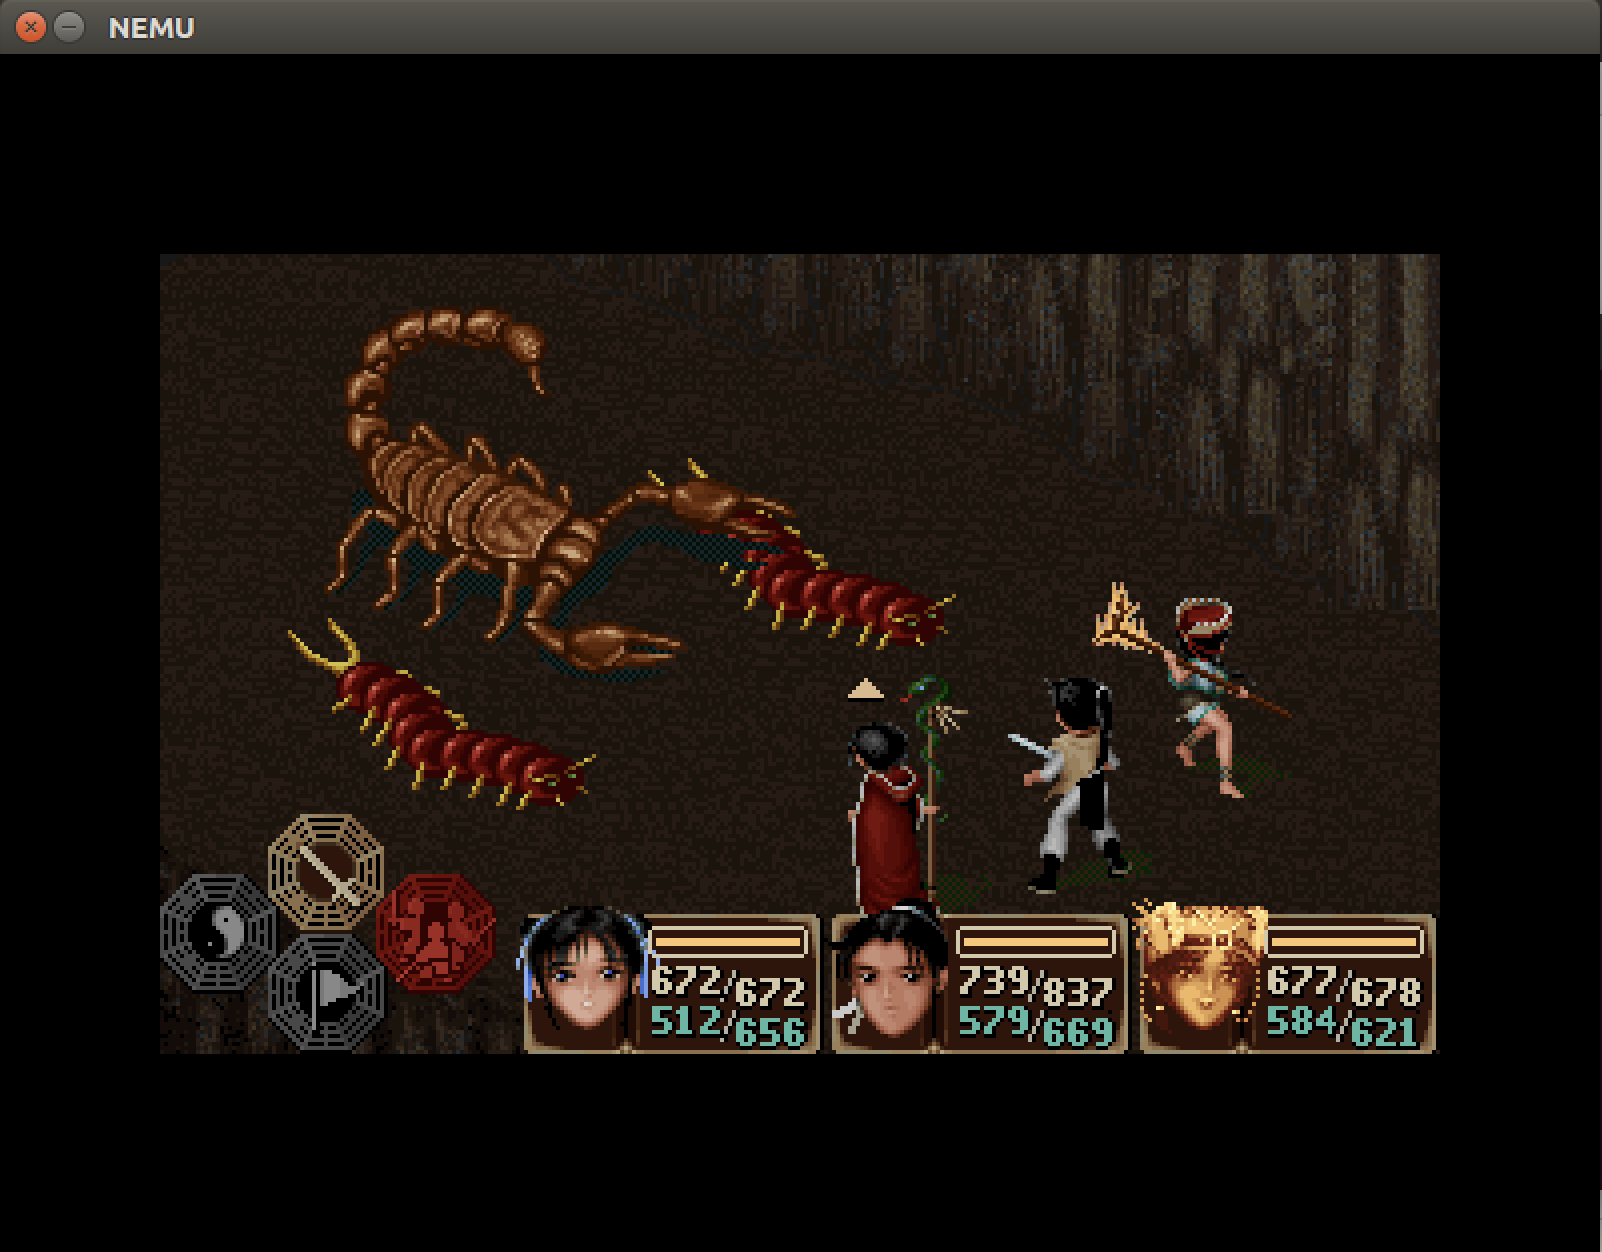
\includegraphics[width=0.46\textwidth]{pa5-battle-1.png}
  }
  \subfigure[战斗过程画面]{
    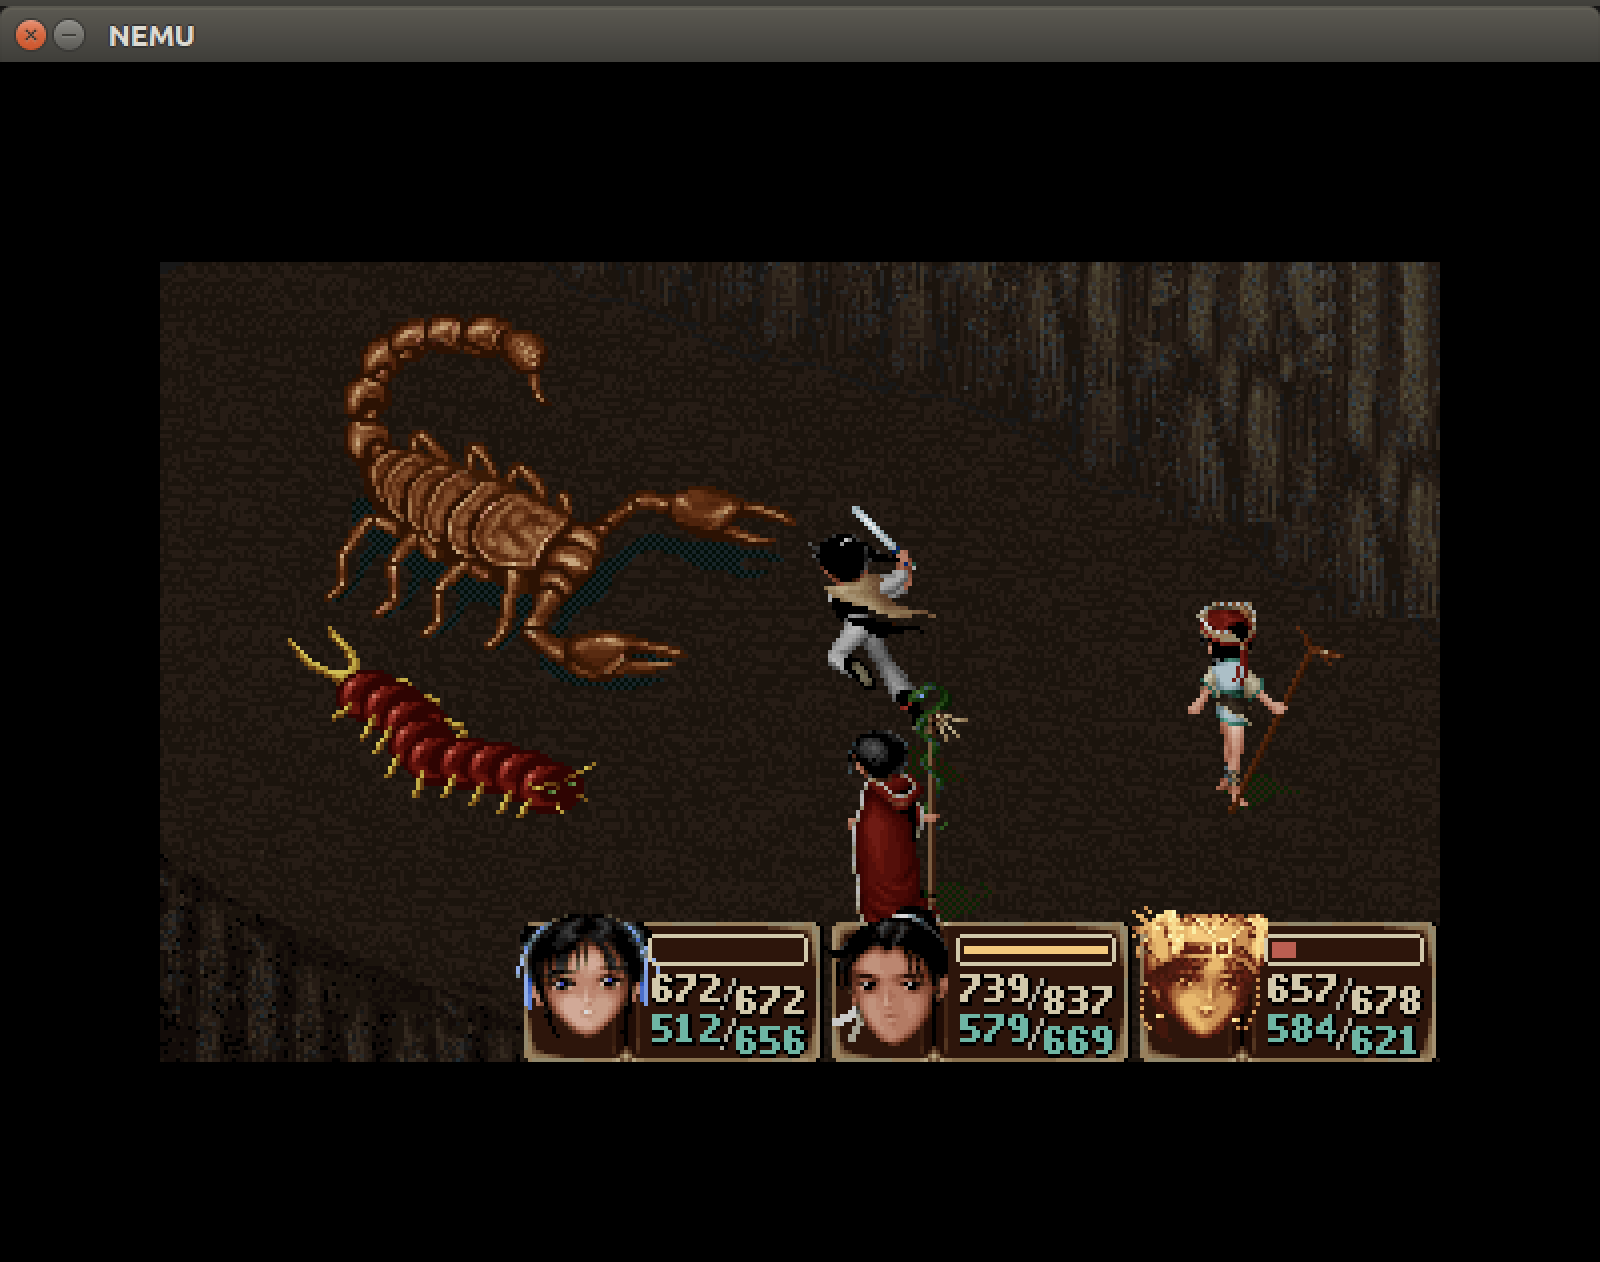
\includegraphics[width=0.46\textwidth]{pa5-battle-2.png}
  }
  \caption{战斗验证结果}
\end{figure}

\begin{figure}[H]
  \centering
  
\includegraphics[width=0.52\textwidth]{pa5-battle-monster.png}
  \caption{战斗场景中的敌方画面}
\end{figure}

从验证角度看，这一阶段可以得到一个比较明确的结论：\texttt{FLOAT / binary scaling} 的功能主线已经跑通，\texttt{pal} 不再停留在初始化阶段，而是能够真正进入战斗逻辑。

\section{perf 分析与局部性能优化}

\subsection{为什么开始做性能分析}
在把 \texttt{PA4} 遗留下来的多进程调度收缩回单进程 \texttt{pal} 之后，运行速度依然很慢。此时继续凭经验猜测“是不是某个函数太慢”意义不大，因此这一阶段先转向 \texttt{perf}，观察系统把时间真正花在了哪里。由于战斗阶段推进比较慢，最先能稳定拿到的是从游戏启动到 \texttt{PAL\_InitResources success} 这一段，因此第一轮采样就固定在 \texttt{pal} 初始化阶段。

\subsection{第一轮 \texttt{perf} 采样方法}
远端虚拟机安装好 \texttt{perf} 之后，实际采样时采用了固定时间窗口的方法：

\begin{lstlisting}[language=bash]
printf "c\n" | timeout 25s perf record -F 99 -g \
  -o /tmp/pa5-pal.perf.data \
  ./nemu/build/nemu ./nanos-lite/build/nanos-lite-x86-nemu.bin
\end{lstlisting}

这里的做法是让 \texttt{nemu} 自动运行 25 秒，并用 \texttt{-F 99} 以固定频率采样调用栈。之所以不直接测战斗阶段，是因为当时游戏推进很慢，先采启动与资源加载阶段反而更容易获得稳定、可重复的样本。

\subsection{第一轮热点分析结果}
第一轮 \texttt{perf} 结果很集中，热点主要分布在访存辅助路径上：

\begin{table}[H]
  \centering
  \begin{tabular}{lc}
    \toprule
    符号 & Self 占比 \\
    \midrule
    \texttt{is\_mmio} & 18.40\% \\
    \texttt{page\_translate.part.1} & 13.83\% \\
    \texttt{paddr\_read} & 12.52\% \\
    \texttt{\_\_memcpy\_sse2\_unaligned} & 11.17\% \\
    \texttt{paddr\_write} & 9.09\% \\
    \texttt{vaddr\_read} & 6.60\% \\
    \texttt{exec\_real} & 4.19\% \\
    \bottomrule
  \end{tabular}
  \caption{第一轮 perf 主要热点}
\end{table}

这张表非常关键，因为它直接说明当前性能瓶颈并不主要在 \texttt{pal} 自己的上层逻辑，而在 \texttt{NEMU} 的访存链条上：每次客户机访问虚拟地址，都要经过 \texttt{vaddr\_read}、页表翻译、物理读写和 \texttt{MMIO} 判断。初始化阶段资源文件又比较多，\texttt{\_\_memcpy\_sse2\_unaligned} 也因此进入了高位。

\subsection{围绕热点做的局部优化}
有了第一轮结果之后，后续优化不再盲改，而是围绕热点逐项推进。

第一项优化是给 \texttt{is\_mmio()} 加快路径。原始实现每次都线性扫描所有 \texttt{MMIO} 区间：

\begin{lstlisting}[language=C]
int is_mmio(paddr_t addr) {
  int i;
  for (i = 0; i < nr_map; i ++) {
    if (addr >= maps[i].low && addr <= maps[i].high) {
      return i;
    }
  }
  return -1;
}
\end{lstlisting}

而当前实验环境下 \texttt{MMIO} 区域数量很少，因此这里先加了 \texttt{nr\_map==0} 和 \texttt{nr\_map==1} 的快路径，并额外试过“排序 + 二分查找”和“页级查表”两种做法。最后留下的是更稳的排序与二分版本，因为它虽然收益不算大，但实现简单，而且没有引入额外波动。

第二项优化是减少页表项的重复写回。原始 \texttt{page\_translate()} 每次都会无条件回写 \texttt{PDE/PTE} 的 \texttt{A/D} 位：

\begin{lstlisting}[language=C]
pde.accessed = 1;
paddr_write(..., pde.val);
pte.accessed = 1;
if (is_write) pte.dirty = 1;
paddr_write(..., pte.val);
\end{lstlisting}

后面改成“只有位从 0 变成 1 时才写回”，这样可以直接减少 \texttt{paddr\_write} 的调用次数。实际结果里 \texttt{paddr\_write} 的占比确实从 9\% 左右下降到了 7\% 左右，说明这一改动是有效的。

第三项优化是去掉无意义的重复检查和调试输出。这里包括：

\begin{itemize}
  \item 没有 watchpoint 时，不再每条指令都调用 \texttt{check\_watchpoints()}
  \item 暂时关掉 \texttt{fs\_open}、\texttt{schedule}、\texttt{do\_event time} 等高频 \texttt{Log()}
\end{itemize}

这类改动本身不改变执行模型，但能避免分析结果被调试辅助路径污染。

\subsection{局部优化前后的 \texttt{perf} 对比}
围绕访存链和日志做完第一轮局部优化之后，这里只保留“优化前”和“最终保留方案”两组结果，而不把 \texttt{TB} 与 \texttt{JIT} 混进来。这样处理的原因很直接：这一节的目标只是说明基础热点修补是否有效；\texttt{TB} 和 \texttt{JIT} 属于后面的执行模型改造，应当放回各自章节单独分析。

\begin{table}[H]
  \centering
  \begin{tabular}{lcc}
    \toprule
    热点符号 & 优化前 & 优化后 \\
    \midrule
    \texttt{is\_mmio} & 18.39\% & 18.40\% \\
    \texttt{paddr\_read} & 18.10\% & 17.99\% \\
    \texttt{page\_translate} & 15.46\% & 15.02\% \\
    \texttt{paddr\_write} & 9.09\% & 7.78\% \\
    \texttt{vaddr\_read} & 9.72\% & 8.91\% \\
    \bottomrule
  \end{tabular}
  \caption{局部优化前后的 \texttt{perf} 对比}
\end{table}

这张表里最重要的信息有两点。第一，\texttt{A/D} 位条件回写对 \texttt{paddr\_write} 的下降是有效的，这说明页表项重复写回确实是可以消掉的一部分冗余开销。第二，\texttt{is\_mmio()}、\texttt{paddr\_read} 和 \texttt{page\_translate} 虽然也有所下降，但变化幅度不大，说明局部热点修补可以把系统往前推一截，却还不足以从根本上改写解释执行的成本结构。

这一轮对比反映的是一个比较朴素的结论：局部修补确实能让 \texttt{page\_translate}、\texttt{paddr\_write} 和一部分访存辅助路径略有下降，但它并没有改变主瓶颈仍然集中在访存链上的事实。也就是说，靠这类热点小修可以把系统往前推一截，但很难从根上改变解释执行的成本结构。

\subsection{全初始化阶段的 opcode 频率统计}
为了进一步判断哪些指令最值得优先放进 \texttt{TB/JIT}，后面又对整个 \texttt{pal} 初始化阶段做了一次 opcode 频率统计。统计范围从游戏启动到 \texttt{PAL\_InitResources success}，总共记录了约 426 万条客户机指令。结果显示，真正的高频 opcode 主要集中在移动、比较和条件跳转上：

\begin{table}[H]
  \centering
  \begin{tabular}{lcc}
    \toprule
    opcode & 语义示意 & 占比 \\
    \midrule
    \texttt{89} & \texttt{mov r32 -> r/m32} & 25.06\% \\
    \texttt{39} & \texttt{cmp r32, r/m32} & 13.38\% \\
    \texttt{8b} & \texttt{mov r/m32 -> r32} & 10.95\% \\
    \texttt{83} & 小立即数算术/比较 & 8.18\% \\
    \texttt{75} & \texttt{jnz/jne} & 7.11\% \\
    \texttt{7f} & \texttt{jg} & 5.66\% \\
    \texttt{42} & \texttt{inc edx} & 5.65\% \\
    \texttt{8a} & \texttt{mov r/m8 -> r8} & 5.38\% \\
    \texttt{88} & \texttt{mov r8 -> r/m8} & 5.34\% \\
    \texttt{74} & \texttt{jz/je} & 1.21\% \\
    \bottomrule
  \end{tabular}
  \caption{PAL 初始化阶段全局高频 opcode}
\end{table}

这个统计结果解释了一个之前很容易误判的问题：局部路径里虽然 \texttt{push/pop} 命中很多，但从全局看，它们并不是最值得优先优化的对象。真正占大头的是 \texttt{89/39/8b/83} 和 \texttt{75/74/7f} 这类移动、比较与条件控制流。

\subsection{当前瓶颈总结}
到这一阶段为止，可以对当前性能瓶颈给出比较稳定的判断。第一，访存辅助路径是长期主热点，哪怕前端解释器开销已经下降，它仍然不容易被绕开。第二，\texttt{TB/JIT} 确实能压低前端重复译码和执行框架带来的成本，但若不进一步处理访存链，整体收益就会受到明显限制。第三，后续若继续扩展执行模型，优先级应当放在高频 \texttt{mov/cmp/jcc} 上，而不是继续补边缘指令。

\section{TB 原型实现与效果验证}

\subsection{What is TB？}
\texttt{TB} 是 \texttt{Translation Block}，可以理解成“翻译块”或者“基本块缓存”。解释执行时，客户机每执行一条指令，宿主机都要重新取指、译码、分发，再调用相应 helper。这样做的优点是简单、稳妥，但缺点是同一段客户机代码如果被反复执行，前端分析成本也会被反复支付。

\texttt{TB} 的思路就是：把一小段已经分析过的客户机代码缓存下来，下次再次执行到这段代码时，不再重新完整走一遍前端分析，而是直接复用之前缓存的解析结果。它并不直接生成宿主机机器码，因此比 \texttt{JIT} 更保守；但它已经足以把重复译码的成本压下去，因此很适合作为进入 \texttt{JIT} 之前的第一步。

\subsection{TB 的数据结构与执行流程}
当前实现使用一个 direct-mapped 的最小 \texttt{TB} cache，以 \texttt{cpu.eip} 为索引，缓存一段 basic block 中每条客户机指令的起始地址、opcode 和下一条地址。数据结构可以概括为：

\begin{lstlisting}[language=C]
#define TB_CACHE_SIZE 4096
#define TB_MAX_INSTR 32

typedef struct {
  vaddr_t pc;
  uint8_t opcode;
  vaddr_t next_eip;
} TBInstr;

typedef struct {
  bool valid;
  vaddr_t start_eip;
  int nr_instr;
  TBInstr instr[TB_MAX_INSTR];
} TBEntry;
\end{lstlisting}

这套结构的思路是：第一次从某个 \texttt{EIP} 开始执行时，仍然走原来的解释路径，同时顺手把这段 block 里的指令信息记录下来；下一次再遇到相同的 \texttt{EIP}，就不必重新做一轮完整的取指和 opcode 分发，而是直接复用缓存条目。当前实现中，\texttt{TB} 并没有试图跨越所有控制流边界，而是在遇到跳转、前缀指令或其它不稳定点时提前截断 block。这种保守策略虽然降低了 block 长度，但明显提高了原型的稳定性。

真正把 \texttt{TB} 接进执行路径的入口在 \texttt{cpu\_exec()} 一侧。这里的核心不是“写了一个新循环”，而是在原来的解释执行框架前面插入一次 \texttt{TB} 查询：若当前 \texttt{EIP} 命中缓存，则按 \texttt{TBInstr} 中记录的 opcode 顺序回放；若未命中，则先进入普通解释路径，同时构造一条新的 \texttt{TBEntry}。简化后的关键流程如下：

\begin{lstlisting}[language=C]
TBEntry *tb = tb_lookup(cpu.eip);
if (tb != NULL && tb->valid) {
  exec_wrapper_cached(tb);
} else {
  tb = tb_build(cpu.eip);
  exec_wrapper_cached(tb);
}
\end{lstlisting}

这里的 \texttt{exec\_wrapper\_cached()} 并不是“绕开执行语义”，而只是跳过了重复的 opcode 取指和表查询。每条客户机指令仍然会真正执行，设备更新和中断检查也仍然保留，因此当前这版 \texttt{TB} 依然是一个“保守但稳定”的优化。

\subsection{TB 的验证方法}
验证 \texttt{TB} 的方法没有直接依赖游戏画面，而是固定执行同样数量的客户机指令，再比较 wall time。这样做有两个好处：一是避免不同游戏推进阶段带来的随机性；二是更容易把改动与吞吐量直接对应起来。

实际对比时，使用的是同一份 \texttt{nanos-lite} 镜像，只替换 \texttt{NEMU} 的执行逻辑。固定命令为：

\begin{lstlisting}[language=bash]
si 20000000
\end{lstlisting}

也就是让模拟器稳定执行 2000 万条客户机指令，再记录总耗时，并换算成 \texttt{M guest instr/s}。

\subsection{TB 的吞吐量测试结果}
对比结果如下：

\begin{table}[H]
  \centering
  \begin{tabular}{lccc}
    \toprule
    版本 & 平均耗时 & 吞吐量 & 相对提升 \\
    \midrule
    pre-TB baseline & 2.415s & 8.28 M instr/s & - \\
    TB & 2.085s & 9.59 M instr/s & +15.8\% \\
    \bottomrule
  \end{tabular}
  \caption{TB 相对 pre-TB baseline 的吞吐量对比}
\end{table}

这组数据说明，哪怕还没有真正进入 \texttt{JIT}，仅仅是把一段已经分析过的客户机指令缓存下来，就已经能给解释执行带来明确收益。从 \texttt{perf} 的角度看，这一收益也能对应到 \texttt{exec\_real} 占比的大幅下降。

\subsection{TB 阶段的 \texttt{perf} 变化}
为了验证 \texttt{TB} 带来的收益确实来自解释前端，而不是样本误差，这里又单独对 \texttt{TB only} 做了一轮 \texttt{perf}。对比最早的干净基线，可以看到：

\begin{table}[H]
  \centering
  \begin{tabular}{lcc}
    \toprule
    热点符号 & 早期基线 & TB only \\
    \midrule
    \texttt{is\_mmio} & 18.39\% & 19.60\% \\
    \texttt{paddr\_read} & 18.10\% & 16.29\% \\
    \texttt{page\_translate} & 15.46\% & 14.54\% \\
    \texttt{vaddr\_read} & 9.72\% & 7.88\% \\
    \texttt{exec\_real} & 6.71\% & 0.78\% \\
    \texttt{exec\_wrapper\_cached} & - & 7.35\% \\
    \bottomrule
  \end{tabular}
  \caption{TB only 与早期基线的 perf 对比}
\end{table}

这张表里最显眼的变化是 \texttt{exec\_real} 从 6\% 以上下降到了不到 1\%。这说明 \texttt{TB} 已经明显减少了前端重复译码和执行分发的成本。不过与此同时，\texttt{is\_mmio}、\texttt{page\_translate} 和 \texttt{paddr\_read} 仍然稳居高位，这也意味着 \texttt{TB} 虽然有效，但它并没有碰到真正最重的访存主链。

\subsection{TB 大小探究}
在 \texttt{TB} 基本跑通之后，又额外做了一次关于 block 最大长度的探究。这里固定其它条件不变，只修改 \texttt{TB\_MAX\_INSTR}，观察吞吐量如何变化。结果如下图所示：

\begin{figure}[H]
  \centering
  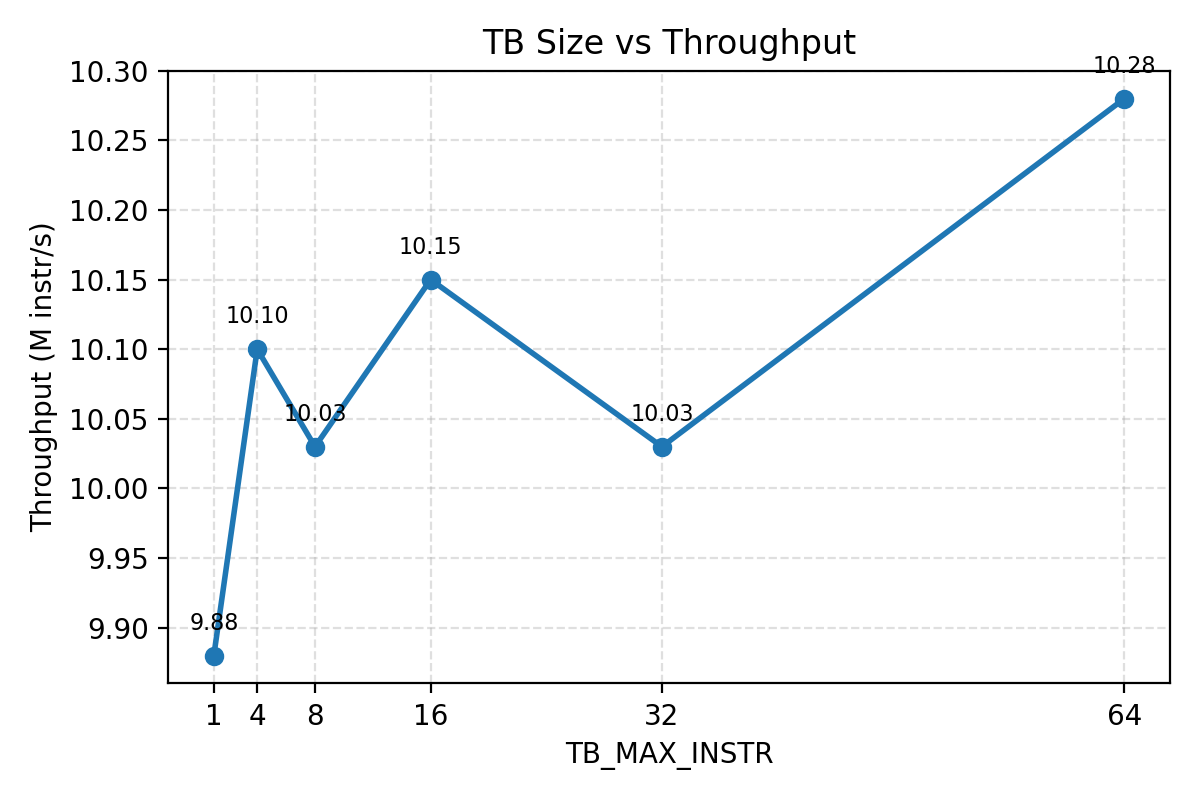
\includegraphics[width=0.62\textwidth]{tb-size-throughput.png}
  \caption{不同 TB 最大长度下的吞吐量}
\end{figure}

对应数据为：

\begin{table}[H]
  \centering
  \begin{tabular}{ccccccc}
    \toprule
    \texttt{TB\_MAX\_INSTR} & 1 & 4 & 8 & 16 & 32 & 64 \\
    \midrule
    吞吐量 / M instr/s & 9.88 & 10.10 & 10.03 & 10.15 & 10.03 & 10.28 \\
    \bottomrule
  \end{tabular}
  \caption{TB 大小与吞吐量的关系}
\end{table}

这组结果说明，\texttt{TB} 不是越长越一定更好。长度只有 1 时，收益最差，因为每条客户机指令都要重新查一次 cache，几乎退化回解释器；长度增加到 16、32、64 后，吞吐量差距已经不大，说明 block 足够大之后，前端缓存带来的收益开始变平。虽然这组实验里 \texttt{64} 的吞吐量最高，但最终仍保留了更保守的 \texttt{32}，原因是它和 \texttt{64} 差距不大，而当前 \texttt{TB} 原型仍然比较粗糙，保守一点更有利于稳定性。

\subsection{TB 阶段结论}
到这一阶段，\texttt{TB} 已经具备了比较完整的闭环：功能上能稳定运行，性能上能带来约 15\% 的吞吐量提升，还额外完成了 block 大小的探究。因此后面的 \texttt{JIT} 尝试并不是从空白开始，而是建立在一个已经有正收益的 \texttt{TB} 基础之上。

\section{JIT 尝试实现及分析}

\subsection{什么是 JIT}
\texttt{JIT} 是 \texttt{Just-In-Time compilation}，也就是“即时编译”。如果说解释执行是在每条客户机指令到来时都重新分析它一次，那么 \texttt{JIT} 的想法就是：把一部分客户机代码临时翻译成宿主机代码，下次再执行到这里时直接运行翻译结果，而不是每次都重新解释。

在这个意义上，\texttt{TB} 和 \texttt{JIT} 的关系可以概括为：\texttt{TB} 是“缓存已分析的客户机代码”，而 \texttt{JIT} 是“生成可直接执行的宿主机代码”。前者主要减少重复取指和重复分发，后者理论上可以进一步减少 helper 和解释器前端的往返。因此这次实验中，\texttt{JIT} 不是替代 \texttt{TB}，而是建立在 \texttt{TB} 已经跑通之后的一层继续探索。

这里需要先说明一个边界：本次实现并不是完整框架的 \texttt{JIT}，而是基于 \texttt{JIT} 思路做的简化版原型。完整 JIT 要真正形成稳定收益，至少还需要系统处理寄存器映射、\texttt{EFLAGS} 维护、block 间链接、访存 codegen、中断与异常的一致性，以及代码缓存失效等问题。对于当前这份 \texttt{NEMU} 而言，这已经不是“继续补几条 opcode”可以解决的，而是在重写执行模型。

因此这里选择的策略更保守：仍然以 \texttt{TB} 为基本单位，只在极小白名单范围内，为少量高频且相对安全的客户机指令生成宿主机代码；其余情况一律回退到 \texttt{TB} 或解释执行。这样做的目标不是把 \texttt{pal} 全部变成 JIT 运行，而是验证两件事：第一，当前环境下“生成并执行宿主机代码”这条链是可行的；第二，局部 JIT 在真实 workload 上是否能够带来可测的收益。

\subsection{JIT 的实现}
当前这版实现并没有绕开 \texttt{TB}，而是把 \texttt{JIT} 当成 \texttt{TB} 命中后的进一步优化。换句话说，先由 \texttt{TB} 决定“这段客户机代码是否已经缓存过”，再由 \texttt{JIT} 决定“缓存中的某条指令是否替换成宿主机代码执行”。因此它的结构不是“解释器”和“JIT”二选一，而是：

\begin{center}
\texttt{解释执行} $\rightarrow$ \texttt{TB cache} $\rightarrow$ \texttt{局部 JIT}
\end{center}

这一层关系在 \texttt{cpu-exec.c} 中直接体现在 \texttt{TBEntry} 结构上。当前 \texttt{TBEntry} 除了保存 \texttt{TBInstr} 外，还额外保存了每条客户机指令对应的宿主机函数指针、代码缓冲区，以及该条 JIT 指令是否自己维护 \texttt{EIP}：

\begin{lstlisting}[language=C]
typedef struct {
  bool valid;
  vaddr_t start_eip;
  int nr_instr;
  TBInstr instr[TB_MAX_INSTR];
#if ENABLE_JIT_SANDBOX
  void (*jit_fn[TB_MAX_INSTR])(void);
  void *jit_buf[TB_MAX_INSTR];
  bool jit_owns_eip[TB_MAX_INSTR];
#endif
} TBEntry;
\end{lstlisting}

\texttt{TB} 被提交到缓存后，如果某条指令的 \texttt{pc} 落在允许的白名单范围里，就会尝试为它生成宿主机代码：

\begin{lstlisting}[language=C]
TBEntry *slot = &tb_cache[tb_hash(tb_building.start_eip)];
*slot = tb_building;
#if ENABLE_JIT_SANDBOX
for (int i = 0; i < slot->nr_instr; i++) {
  if (jit_cacheable_pc(slot->instr[i].pc)) {
    if (!tb_try_build_jit(slot, i)) {
      jit_opcode_miss[slot->instr[i].bytes[0]]++;
    }
  }
}
#endif
\end{lstlisting}

也就是说，当前 JIT 的构建时机并不是“运行到一条指令时再现场编译”，而是在 \texttt{TB} 缓存形成之后顺手扫描 block 内每条指令，能翻的就先翻成宿主机代码，翻不了就继续保留为普通 \texttt{TB} 指令。

真正执行时，\texttt{cpu\_exec()} 会先命中 \texttt{TB}，再决定这一条 \texttt{TBInstr} 是否调用宿主机代码：

\begin{lstlisting}[language=C]
if (tb->jit_fn[i] != NULL && jit_cacheable_pc(tb->instr[i].pc)) {
  jit_exec_count++;
  jit_record_hit(&tb->instr[i]);
  tb->jit_fn[i]();
  owns_eip = tb->jit_owns_eip[i];
  if (!owns_eip) {
    cpu.eip = tb->instr[i].next_eip;
  }
} else {
  exec_wrapper_cached(tb->instr[i].opcode, false);
}
\end{lstlisting}

这个分支很能体现当前原型的定位：JIT 不是去重写整个执行循环，而是只在单条客户机指令已经成功构建出宿主机代码时才接管；一旦没构建成功，或者不在白名单内，就立即退回 \texttt{TB} 的缓存回放路径。

\subsection{最小 JIT 沙盒测试}
为了避免一上来就在 \texttt{pal} 上把整个执行链打坏，这里先写了一个极小测试程序 \texttt{jitmini}，只包含非常有限的指令形式，如 \texttt{mov imm32, reg}、寄存器间 \texttt{mov} 和 \texttt{nop}。与此同时，在 \texttt{cpu-exec.c} 中增加了默认关闭的 \texttt{ENABLE\_JIT\_SANDBOX} 开关，以及一套最小宿主机代码生成逻辑。

这一阶段的重点不是追求性能，而是证明以下几件事：

\begin{itemize}
  \item 可以为客户机指令生成宿主机机器码
  \item 生成后的代码可以通过 \texttt{mmap(PROT\_EXEC)} 的缓冲区执行
  \item 执行结果能正确反映到 \texttt{cpu.gpr[]} 等客户机状态上
\end{itemize}

\texttt{jitmini} 跑到 \texttt{GOOD TRAP}，说明最小 \texttt{JIT} 沙盒本身是通的。

这一步里最关键的不是“开了一个宏”，而是先把最小 codegen 链闭合起来。当前实现会先判断某条客户机指令是否属于受支持的安全集合；若属于，就为它生成一段宿主机机器码，写到可执行缓冲区中；随后把这段机器码当函数调用。简化后的结构如下：

\begin{lstlisting}[language=C]
if (jit_can_translate(pc, opcode)) {
  uint8_t *buf = jit_emit_begin();
  jit_emit_insn(buf, pc, opcode, modrm, imm);
  jit_emit_end(buf);
  jit_entry->fn = (jit_fn_t)buf;
}
\end{lstlisting}

这里的 \texttt{jit\_emit\_insn()} 并没有试图把整个 x86 子集一次性翻完，而是只处理极少数最简单的形式，例如 \texttt{mov imm32, reg}、寄存器间 \texttt{mov} 和 \texttt{nop}。这样做的目的不是追求覆盖率，而是先确认“宿主机代码生成并执行”这件事本身是可行的。

当前这版 JIT 并不是“完整地把一条客户机指令翻译成纯宿主机逻辑”，而是保守地分成两层。对于最简单的寄存器操作，会直接生成宿主机机器码去读写 \texttt{cpu.gpr[]}；对于稍复杂、但又希望先保证正确性的情况，则仍然保留 helper 参与。

例如 \texttt{test r32, r32} 这类指令，当前实现不是自己在机器码里维护全部 \texttt{EFLAGS}，而是把寄存器号压栈，再调用 helper：

\begin{lstlisting}[language=C]
emit8(&p, 0x6A); emit8(&p, rm);
emit8(&p, 0x6A); emit8(&p, reg);
emit_call_rel32(&p, (uintptr_t)jit_helper_test_rr);
emit8(&p, 0x83); emit8(&p, 0xC4); emit8(&p, 0x08);
\end{lstlisting}

对应的 helper 再去更新标志位：

\begin{lstlisting}[language=C]
static void jit_helper_test_rr(int dst, int src) {
  uint32_t val = reg_l(dst) & reg_l(src);
  cpu.ZF = (val == 0);
  cpu.SF = (val >> 31) & 1;
  cpu.CF = 0;
  cpu.OF = 0;
}
\end{lstlisting}

条件跳转和最小 \texttt{call/ret} 也是类似做法。比如短条件跳转 \texttt{jcc} 不会在宿主机代码里完成全部控制流逻辑，而是把 \texttt{target}、\texttt{fallthrough} 和 opcode 交给 helper：

\begin{lstlisting}[language=C]
emit_push_imm32(&p, (uint32_t)target);
emit_push_imm32(&p, (uint32_t)fallthrough);
emit_push_imm8(&p, op);
emit_call_rel32(&p, (uintptr_t)jit_helper_jcc_short);
emit_add_esp_imm8(&p, 0x0c);
tb->jit_owns_eip[idx] = true;
\end{lstlisting}

这套设计的优点是实现快、调试容易，而且能把最危险的状态更新统一放回 C helper 处理；缺点也同样明显：宿主机代码虽然生成出来了，但每条客户机指令往往还要绕回 helper 和原执行框架，因此收益天然会被稀释。这也是后面性能分析里，JIT 能继续压低一部分前端开销，却始终很难明显超过 \texttt{TB only} 的直接原因。

\subsection{\texttt{jitmini} 上的受控 benchmark}
为了进一步回答“这套最小 JIT 到底有没有性能价值”，把测试内容改成了一个纯寄存器小循环，只保留当前 JIT 已支持的简单指令：

\begin{lstlisting}[language=C]
asm volatile(
    "movl $10000000, %%ecx\n\t"
    "1:\n\t"
    "movl $0x12345678, %%eax\n\t"
    "movl %%eax, %%ebx\n\t"
    "test %%ebx, %%ebx\n\t"
    "jz 2f\n\t"
    "sub $1, %%ecx\n\t"
    "jnz 1b\n\t"
    "2:\n\t"
    "movl %%ebx, %0\n\t"
    : "=m"(sink)
    :
    : "eax", "ebx", "ecx", "cc");
\end{lstlisting}

这段代码的作用不是模拟真实游戏逻辑，而是构造一个“几乎不受访存链影响”的受控工作负载，让 JIT 的前端收益能够更直接地体现出来。实际测得结果如下：

\begin{table}[H]
  \centering
  \begin{tabular}{lccc}
    \toprule
    版本 & 运行 1 & 运行 2 & 平均耗时 \\
    \midrule
    TB only & 6.88s & 6.61s & 6.745s \\
    JIT on & 1.07s & 1.06s & 1.065s \\
    \bottomrule
  \end{tabular}
  \caption{\texttt{jitmini} 上 TB only 与 JIT on 的耗时对比}
\end{table}

按平均值计算，JIT 在这个受控小程序上大约带来了 \texttt{6.3x} 的加速。日志中还能看到大量真实命中：

\begin{lstlisting}
[jit-sandbox] summary built=63 executed=59999990
[jit-sandbox] opcode 74 hits=9999998
[jit-sandbox] opcode 75 hits=9999999
[jit-sandbox] opcode 83 hits=9999999
[jit-sandbox] opcode 85 hits=9999998
[jit-sandbox] opcode 89 hits=9999998
[jit-sandbox] opcode b8 hits=9999998
\end{lstlisting}

这组结果非常重要。它说明 JIT 思路本身并没有问题：在一个足够受控、几乎不受分页和 MMIO 影响的小程序上，即时编译确实可以明显快于 \texttt{TB only}。后面在 \texttt{pal} 上收益收敛，并不是因为 JIT 完全无效，而是因为真实 workload 的主瓶颈并不只在前端解释层。

\subsection{在\texttt{pal}上测试JIT}
在前面的测试跑通之后，没有直接把 \texttt{JIT} 开到整个 \texttt{pal}，而是采用白名单策略，从 \texttt{PAL\_MKFGetChunkCount}、\texttt{PAL\_MKFGetChunkSize}、\texttt{PAL\_MKFReadChunk} 等资源处理函数开始。选择这几段路径的原因是：它们属于真实 workload，但控制流和数据流相对可控，比战斗主循环和图形更新更适合作为第一批试验对象。

\subsection{逐步扩大支持的指令}
接下来并不是一次性上很多 opcode，而是按“先安全、后复杂”的顺序逐步扩展。最开始只支持：

\begin{itemize}
  \item \texttt{mov imm32, r32}
  \item \texttt{mov r32, r32}
  \item \texttt{nop}
\end{itemize}

随后逐步加入：

\begin{itemize}
  \item \texttt{test r32, r32}
  \item \texttt{83} 组里部分寄存器形式的 \texttt{add/sub/cmp imm8}
  \item \texttt{lea}
  \item \texttt{mov r32, [mem]}
  \item 栈相关指令：\texttt{push/pop/leave}
  \item \texttt{c7}
  \item 扩展 \texttt{89}
  \item 短条件跳转 \texttt{72/74/76/78/75/77/7f}
  \item 最小 \texttt{call/ret}
\end{itemize}

一旦命中白名单扩大得过快，控制流、栈和页表路径就很容易跑偏。比如之前的 \texttt{c7} 一直 miss，最后发现并不是 helper 错了，而是 EA 解析阶段把尾部的 \texttt{imm32} 漏判了；\texttt{jcc} 一开始不命中，也不是条件判断错，而是 \texttt{TB} 对 block 边界的截断策略过于宽松。

就实现方式来看，当前这版 JIT 并不是“完整地把一条客户机指令翻成纯宿主机逻辑”，而是保守地分成两类。对于最简单的寄存器操作，会直接生成宿主机机器码去读写 \texttt{cpu.gpr[]}；对于稍复杂、但又希望先验证正确性的情况，则仍然保留 helper 参与。例如 \texttt{test r32, r32} 这类指令，当前实现会显式更新 \texttt{ZF/SF/CF/OF} 等标志位：

\begin{lstlisting}[language=C]
static void jit_helper_test_rr(int dst, int src) {
  uint32_t val = reg_l(dst) & reg_l(src);
  cpu.ZF = (val == 0);
  cpu.SF = (val >> 31) & 1;
  cpu.CF = 0;
  cpu.OF = 0;
}
\end{lstlisting}

而像 \texttt{lea} 这样的地址计算，则属于“不真正访存、但能带来真实 workload 覆盖”的比较合适对象，因此也被单独纳入了当前白名单。换句话说，这一阶段的实现策略不是“追求一次性变成完整 JIT”，而是先把最安全、最常见、最有价值的一小批 opcode 接进来。

\subsection{命中统计与吞吐量变化}
JIT 扩展过程中，前后其实做过两类性能测试。第一类是前面 \texttt{jitmini} 的受控 benchmark，用来说明“在几乎不受访存链影响的小程序上，JIT 思路本身确实能明显加速”；第二类则是把真实 \texttt{pal} 镜像放在固定的大工作量下，比较 \texttt{pre-TB baseline}、\texttt{TB only} 和当前局部 JIT 的整体耗时。

先看这一组更适合作为最终背书的长跑数据。这里固定执行：

\begin{center}
\texttt{si 400000000}
\end{center}

也就是让模拟器稳定执行 4 亿条客户机指令，再比较不同执行模型的 wall time。结果如下：

\begin{table}[H]
  \centering
  \begin{tabular}{lccc}
    \toprule
    版本 & 总耗时 & 吞吐量 & 说明 \\
    \midrule
    pre-TB baseline & 45.75s & 8.74 M instr/s & 纯解释执行 \\
    TB only & 36.79s & 10.87 M instr/s & 前端缓存已分析指令 \\
    当前局部 JIT & 40.74s & 9.82 M instr/s & 在 TB 上叠加简化版 JIT \\
    \bottomrule
  \end{tabular}
  \caption{固定执行 4 亿条客户机指令时的吞吐量对比}
\end{table}

这组数据给出的结论非常直接。第一，\texttt{TB} 相比最早的纯解释执行版本有稳定收益，这与前面的 \texttt{perf} 变化完全一致；第二，当前这版局部 JIT 虽然仍然比最早 baseline 快，但已经明显慢于 \texttt{TB only}。因此这里最重要的现象不是“JIT 有没有命中”，而是“命中了之后，为什么整体吞吐量仍然没有超过 TB”。

前面做过的阶段性测试仍然有意义，因为它能展示收益变化的趋势：最开始白名单很窄时，JIT 框架本身的额外成本抵不过它带来的收益，因此总体甚至比 \texttt{TB only} 更慢；随着 \texttt{test}、\texttt{83}、\texttt{8d}、\texttt{8b} 等高频指令逐步接入，局部阶段一度出现过大约 \texttt{+3.1\%} 的正收益；但继续扩大到更多 \texttt{jcc} 和最小 \texttt{call/ret} 之后，整体又重新回到接近 \texttt{TB only} 的状态。这也说明当前 helper 式 JIT 的收益并不是线性累加的。

\begin{figure}[H]
  \centering
  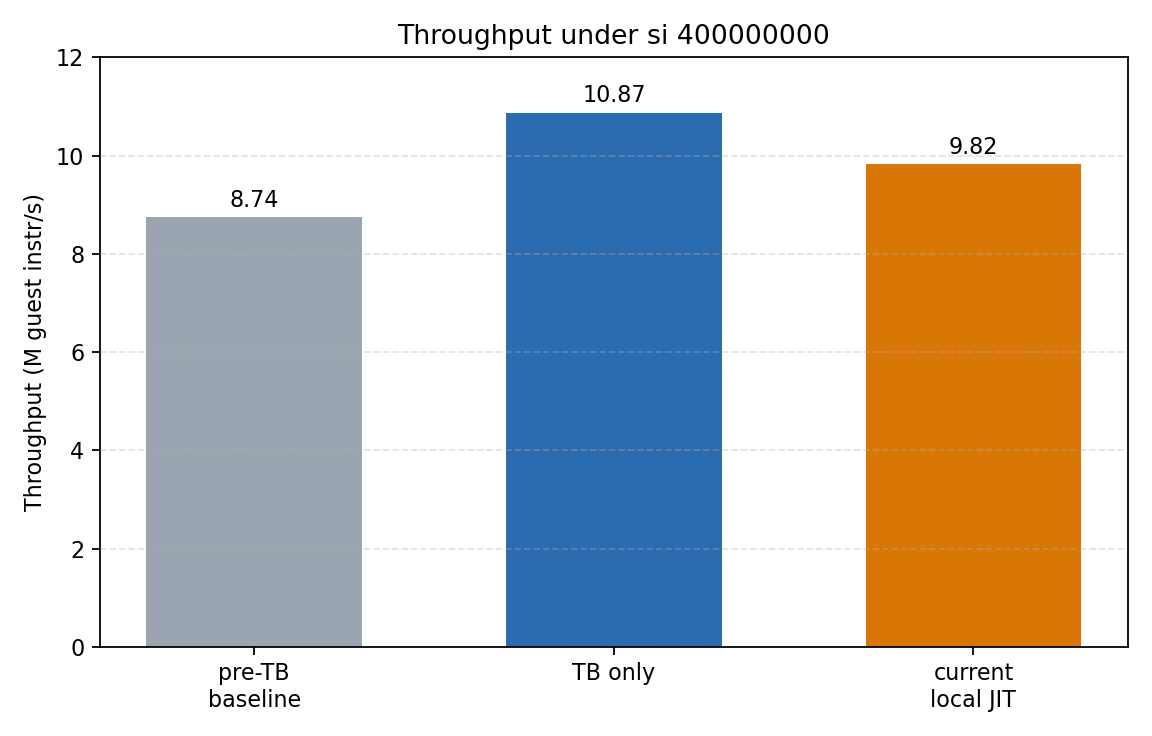
\includegraphics[width=0.62\textwidth]{throughput-stages.png}
  \caption{pre-TB、TB 和最佳窄白名单 JIT 的吞吐量对比}
\end{figure}

\subsection{JIT 阶段的 \texttt{perf} 变化}
在当前代码基础上，再把 \texttt{JIT} 打开后，又额外做了一轮 \texttt{perf}，用来和 \texttt{TB only} 对比。结果如下：

\begin{table}[H]
  \centering
  \begin{tabular}{lcc}
    \toprule
    热点符号 & TB only & JIT on \\
    \midrule
    \texttt{is\_mmio} & 19.60\% & 17.68\% \\
    \texttt{paddr\_read} & 16.29\% & 18.17\% \\
    \texttt{page\_translate} & 14.54\% & 14.23\% \\
    \texttt{vaddr\_read} & 7.88\% & 7.93\% \\
    \texttt{exec\_wrapper\_cached} & 7.35\% & 6.34\% \\
    \texttt{exec\_real} & 0.78\% & 1.10\% \\
    \bottomrule
  \end{tabular}
  \caption{TB only 与局部 JIT 开启时的 perf 对比}
\end{table}

从这张表可以看出，\texttt{JIT} 确实继续压低了一部分前端框架成本，例如 \texttt{exec\_wrapper\_cached} 继续下降；但与此同时，\texttt{paddr\_read}、\texttt{page\_translate} 和 \texttt{vaddr\_read} 这类访存热点并没有被根本改写。也就是说，这一阶段的 \texttt{JIT} 更像是在 \texttt{TB} 的基础上继续优化解释前端，而不是已经触碰到了系统真正最重的主瓶颈。

\subsection{为什么 JIT 收益不高，甚至在长跑中慢于 TB}
这一阶段最值得记录的并不是“JIT 已经能支持多少 opcode”，而是为什么继续扩下去之后收益会很快进入平台期，以及为什么在固定执行 4 亿条客户机指令的长跑中，当前局部 JIT 反而慢于 \texttt{TB only}。这里需要先区分两件事：第一，\texttt{jitmini} 这种受控小程序说明 JIT 思路本身是有效的；第二，真实 \texttt{pal} workload 上的收益，取决于当前实现有没有真正绕开系统最重的成本。

当前实现里，所谓 \texttt{JIT} 本质上仍然 heavily 依赖 helper：很多宿主机代码并没有直接把整条客户机语义展开，而是调用 C helper，或者在每条客户机指令之后仍然要回到原执行框架做中断、设备更新和状态维护。这样做的直接后果是：JIT 虽然压掉了一部分前端解释成本，但并没有真正绕开当前系统最重的那条链：

\begin{center}
\texttt{vaddr\_read -> page\_translate -> paddr\_read -> is\_mmio}
\end{center}

前面的 \texttt{perf} 已经证明，长期最重的热点始终停留在访存辅助路径上。因此，局部 \texttt{JIT} 即使扩大了更多 opcode 覆盖，只要这些指令仍然频繁访问内存、仍然频繁落回 helper，收益就很快会被框架开销和访存主链抵消掉。

进一步说，为什么后面扩大白名单之后收益开始变平，其实可以从当前 JIT 的执行方式看出来。现在每条可 JIT 的客户机指令虽然已经替换成宿主机 stub，但：

\begin{itemize}
  \item block 命中仍然先依赖 \texttt{TB} 查找；
  \item 每条指令执行后仍然要回到 \texttt{cpu\_exec()} 的主循环；
  \item 对于 \texttt{test/jcc/call/ret} 等稍复杂指令，宿主机代码内部还会继续调用 helper；
  \item 一旦不在白名单内，或者某条指令构建失败，就立即回退 \texttt{TB}。
\end{itemize}

也就是说，当前这版实现更像是“在 \texttt{TB} 之上插入一些宿主机 stub”，而不是“让一个完整 block 在宿主机上连续执行到底”。白名单继续扩大之后，命中数量虽然变多了，但新的命中并不是纯收益：命中本身会带来额外的 codegen 管理、helper 往返和状态维护成本，因此吞吐量很容易进入平台期。

固定执行 4 亿条客户机指令那组长跑数据把这个问题暴露得更明显。与 \texttt{TB only} 相比，当前局部 JIT 虽然比最早的纯解释执行 baseline 快，但仍然慢于 \texttt{TB only}。原因可以概括为三点：

\begin{enumerate}
  \item \textbf{前端节省的成本还不够大。} 当前 JIT 覆盖的是一批局部高频 opcode，但还没有形成“大段连续宿主机代码直接跑完”的效果。
  \item \textbf{额外管理成本已经开始显现。} 包括白名单判断、\texttt{jit\_fn} 命中检查、\texttt{owns\_eip} 处理、helper 调用和回退逻辑，这些都不是免费的。
  \item \textbf{真实 workload 的主瓶颈仍在访存链。} 即使前端解释层被继续压低，只要 \texttt{paddr\_read}、\texttt{page\_translate}、\texttt{is\_mmio} 这些热点没有被结构性改写，整体吞吐量就很难再往前迈一大步。
\end{enumerate}

因此，当前这版 JIT 的问题不是“方向错了”，而是“还停留在 helper 式、局部覆盖、频繁回退的阶段”。它已经足以证明局部即时编译在 \texttt{pal} 上是可行的，但距离真正能稳定压过 \texttt{TB only} 的完整 JIT，还有明显差距。

\subsection{当前 JIT 的定位}
综上，当前这版 \texttt{JIT} 已经不是玩具空架子。它先在 \texttt{jitmini} 上验证了最小宿主机代码生成链，又在 \texttt{pal} 的真实资源处理路径上完成了从 \texttt{mov/test} 到 \texttt{jcc/call/ret} 的局部扩展，也确实在受控小程序上测到了非常明显的加速。但它仍然不是一个完整高收益的 JIT，更不是已经成熟到可以替代当前 \texttt{TB} 的执行引擎。

更准确的表述应该是：当前已经实现了一个\textbf{基于 JIT 思路的简化版原型}。它的特点是：

\begin{itemize}
  \item 仍然以 \texttt{TB} 为基本缓存单位；
  \item 只在白名单路径上对少量 opcode 生成宿主机代码；
  \item 对 \texttt{test/jcc/call/ret} 等较复杂语义仍然 heavily 依赖 helper；
  \item 只要超出安全范围，就立即退回 \texttt{TB} 或解释执行。
\end{itemize}

因此，这个原型最重要的价值并不是“已经把 \texttt{pal} 彻底 JIT 化”，而是证明了三件事：第一，当前 32 位环境下可以稳定生成并执行宿主机代码；第二，局部 JIT 可以在真实 workload 上获得可观测命中；第三，如果不进一步解决 helper 依赖、block 连续性和访存主链问题，JIT 的收益很快就会到达上限。换句话说，它已经足以作为本次 PA5 的探索性成果，但距离完整框架的 JIT 仍然有明显差距。

\section{思考}

\subsection{为什么解释执行会慢，以及为什么值得继续做 TB/JIT}
指导书后半部分把 \texttt{TB/JIT}、\texttt{Amdahl} 和 \texttt{RTL} 等内容放在一起，核心其实是在引导分析“为什么解释执行会慢，以及为什么更大粒度的执行模型值得尝试”。结合本次实验可以给出比较直接的回答：解释执行的每条客户机指令，都要重新经过取指、译码、分发和 helper 调用，因此前端重复工作很多；\texttt{TB} 的价值在于把一段已经分析过的客户机代码缓存下来，减少重复解析；而 \texttt{JIT} 的进一步目标，则是把客户机代码直接翻译成宿主机代码，尽量绕开解释器前端。不过当前这版原型还没有彻底摆脱 helper，因此它能验证方向可行，却还没有发展成一个足以显著改写整体瓶颈的完整 JIT。

\subsection{为什么 \texttt{FLOAT} 不直接使用真实 \texttt{float}}
指导书这里并不是单纯要求“算出正确数值”，而是要求在当前系统环境里完成一套不依赖硬件浮点的实现。原因在于，这个实验中的 \texttt{NEMU} 和 \texttt{PAL} 用户程序并没有完整的 x87/SSE 浮点支持链。如果直接把所有运算留给真实 \texttt{float}，系统最后并不是在验证“定点数如何支撑应用逻辑”，而是在绕开当前实验真正要补的能力。因此这里使用 \texttt{2\^{}16} 缩放的 fixed-point，不只是为了能算出结果，更是为了在当前简化系统环境下构建一条可控、可验证的数值运算路径。

\subsection{为什么热点会长期停留在访存链}
从多轮 \texttt{perf} 看，无论是纯解释执行、优化后的 \texttt{TB only}，还是开启局部 \texttt{JIT}，真正长期占据高位的始终是 \texttt{is\_mmio}、\texttt{paddr\_read}、\texttt{page\_translate} 和 \texttt{vaddr\_read}。本质原因在于：客户机做一次普通内存访问，在宿主机上并不是“直接读一块数组”，而是要先判断分页是否开启，再走页表翻译，再做物理读写和 MMIO 判断。这类成本几乎附着在所有访存上，因此只靠减少译码前端工作，并不能让这条链自动消失。

\subsection{为什么一个 TB 不应该只对应一条客户指令}
在 \texttt{TB\_MAX\_INSTR} 探究中，最大长度为 1 时吞吐量最差，这个结果很好理解。如果一个 \texttt{TB} 只缓存一条客户机指令，那么每执行一条指令之后都要重新查一次 cache，几乎无法摊薄构建和命中的固定成本。只有当 block 足够长时，前端的取指、opcode 分发和重复判断才能被更多条客户机指令共享，\texttt{TB} 才真正有意义。因此，\texttt{TB} 的价值不在于“缓存一条指令的结果”，而在于“缓存一小段顺序执行的代码”。

\subsection{为什么 helper 式 JIT 收益会平台化}
本次 JIT 原型的一个关键结论是：功能覆盖继续扩大，并不等于吞吐量会持续线性上升。原因在于当前这版 \texttt{JIT} 仍然 heavily 依赖 helper，并且每条客户机指令之后仍然会返回到原来的执行框架。这样做保证了正确性，也降低了把 \texttt{pal} 打坏的风险，但同时意味着它无法像完整 JIT 那样真正绕开原有状态维护和访存路径。因此，局部 JIT 到某个阶段之后，即使能命中更多 \texttt{opcode}，整体收益也会很快进入平台期。

\section{实验过程中遇到的问题与解决方法}
本次实验中比较典型的问题主要有五类。第一类是 \texttt{F\_div\_F()} 触发 \texttt{\_\_divdi3}，这不是公式错了，而是 32 位目标环境下缺少 64 位整除 helper；后面通过手写长除法解决。第二类是 \texttt{FLOAT} 路径暴露出 \texttt{shrd/shld} 未实现，这说明问题已经从应用逻辑延伸到了 NEMU 指令支持层；后面通过补 decode 与执行逻辑解决。第三类是 \texttt{c7} 一直 miss，最后定位到并不是 helper 错，而是 EA 解析对尾部立即数处理不完整。第四类是 \texttt{jcc} 一开始难以稳定命中，排查后发现问题在 block 截断策略，而不是条件判断本身。第五类是 JIT 白名单扩得过快时，控制流和页表路径很容易跑偏，因此后来改成“每扩一类指令都重新短跑验证”的推进方式。

\section{总结}
PA5 最终沿着三条主线完成了推进。第一条主线是定点数实现：\texttt{FLOAT} 相关函数已经补齐，\texttt{pal} 能够真正进入战斗，说明 fixed-point 运算路径已经落地。第二条主线是性能分析与 \texttt{TB}：通过 \texttt{perf} 确认了当前主瓶颈位于访存链，在此基础上实现了最小 \texttt{TB} 原型，并获得了约 15.8\% 的吞吐量提升。第三条主线是 \texttt{JIT} 尝试：先在极小测试程序上验证宿主机代码生成链，再把局部 \texttt{JIT} 推到 \texttt{pal} 真实资源处理路径上，最终实现了一个能局部生效、但收益开始平台化的探索性 \texttt{JIT} 原型。

从实验结果来看，PA5 最重要的收获不只是“又补了几段代码”，而是把功能正确性、性能分析和执行模型改造这三件事第一次比较完整地连在了一起：先让程序正确跑起来，再用测量结果决定优化方向，最后在稳定版本基础上尝试更大的结构性优化。这条推进方式也让后面的系统实验更容易收束成一条清晰主线，而不是停留在零散 patch 的堆积上。

\end{document}
